%!TEX root = ../main.tex
% file: assignment2.tex

\section{Assignment One: Measuring the CPU Time} % (fold)
\label{sec:measuring_the_cpu_time}
Our first goal is to determine whether the Fast Fourier Transform (FFT) package of \emph{numpy} carries a computational time proportional to $\mathcal{O}(n log_2(n))$. The script operates on a set of predetermined random data of base two size, doubling it's size for each iteration. We shall use the \emph{time} module of Python for timing the FFT, then use the method of least squares to determine the expected time. A comparison plot of the FFT timings vs. $\mathcal{O}(n log_2(n))$ is provided.

\subsection{Method} % (fold)
\label{sub:methoda}
To simplify the timing of this project, a class was created for the timer to track executions on our behalf.
\begin{lstlisting}[caption={Timer Class},label=lst:timeclass,firstnumber=1]
    class timer():
\end{lstlisting}
This timer is held within the \emph{objTimer.py} file and reused in various places within the project. Rather than keeping track of timer variables and starting/stopping the timer, we simply call the object which tracks it's own execution.
\begin{lstlisting}[caption={Quantity of Samples to Compute},label=lst:samples,firstnumber=32]
    self.x = x = array([(2**j)*self.start for j in range(self.count+1)])
\end{lstlisting}
The quantity of samples to compute is done by list comprehension as seen in Listing \ref{lst:samples}. The user inputs a start quantity, which is then doubled for a predetermined range. It is then stored within the class as well as locally for use in the function.
\begin{lstlisting}[caption={Random Number Generation},label=lst:rand,firstnumber=36]
    data_seed=rand.random(max(self.x))
\end{lstlisting}
The random numbers are generated prior to the execution of the loop based on the greatest number of samples we wish to compute. This is done in advance to ensure that such random number generation does not pollute our timing results as it may be computationally intensive. Once the random data is generated and our timer object is initialized, we execute the main loop to time our executions.

\begin{lstlisting}[caption={Main Loop Execution},label=lst:mainloop,firstnumber=45]
    for i in x:
        timed()
        for j in range(1,self.loops):
            self.signal=total_signal[:i]
            self.fftCalc(self.signal)
        t = timed()
        self.times.append(t)
\end{lstlisting}
In Listing \ref{lst:mainloop} we iterate over length of the array where \emph{i} is the quantity of samples we wish to take. The object \emph{timed()} is called to zero out the counter and begin counting. The value is not stored as we do not wish to store a zero. We then perform the FFT calculation, and call our timer, \emph{timed()}, once again, this time storing the result to the variable \emph{t}. The times are appended to the list \emph{self.times}, which will be plotted later using \emph{matplotlib}.
\\\\
To then determine whether the data is actually $\mathcal{O}(n \log_2(n))$, we calculated the constant of proportionality, $\alpha$, by finding the value that minimizes the residual sum of squares. This is used to determine what times one would expect for that order and value of $n$.
\\\\
FFT:
\begin{equation}
    ExpectedTime_n=\alpha_1*n*log_2(n)
\end{equation}\noindent
\begin{equation}
    \underset{\alpha_1}{\operatorname{argmin}}
    \sum_{n}(observation_n-\alpha_1*n*log_2(n))^2
\end{equation}\noindent


\begin{lstlisting}[caption={Calculate the expected times},label=lst:expected_times,firstnumber=88]
    def findExact(self):
        """
        Calcuate the raw expected times, then the fitted expected times and plot
        """
        from math import log
        from scipy.optimize import leastsq
        import matplotlib.pyplot as plt
        
        expected = array([log(i,2.0)*i for i in self.x])
        observed = self.times
        def residuals(alpha,observed,expected):
            return observed-alpha*expected
        
        p0=.001
        W = leastsq(residuals,p0,args=(observed,expected), maxfev=100000, full_output=1)
        self.expected_adjusted = [float(W[0]*expected[i]) for i in range(len(expected))]
\end{lstlisting}

% subsection method (end)
\subsection{Results} % (fold)
\label{fig:resultA}
Here we present the results of the method presented in Section~\ref{sub:methoda}. 
\begin{figure}[H]
    \centering
        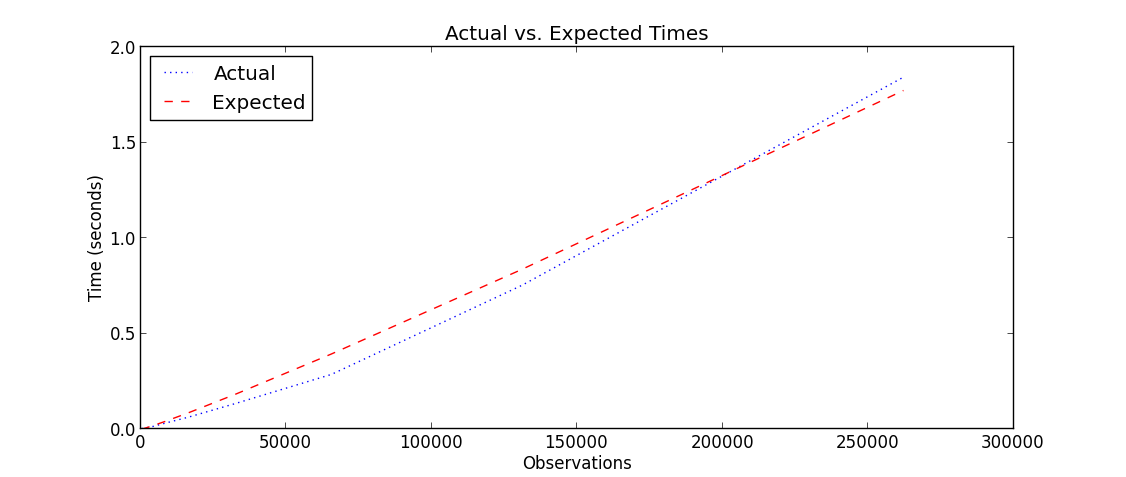
\includegraphics[width=6.5in]{./include/assignment1data.png}
    \caption{Comparison of Actual to Expected Timings}
    \label{fig:exactvsexpt}
\end{figure}\noindent
Figure~\ref{fig:exactvsexpt} depicts a comparison of the experimental times and calculated times. We see that the FFT very closely follows scaling of $\mathcal{O}(n \log_2(n))$. For datasets which are very small, we see faster calculation than predicted; highly likely due to optimization within the algorithm such as cache optimization. Adversely, there are slower than predicted times for larger datasets. Considering the algorithm carries a "best case scenario" of $\mathcal{O}(n \log_2(n))$ this is not of concern.
% subsection results (end)

% section section_name (end)
